\section{Exact Block and Variational Schur Analysis}
\label{app:block_cumulant_analysis}

This appendix derives the linear invariants from the block Lyapunov equation and proves the strong convergence of Galerkin truncations. We do not use Laurent series or covariance inverses.

\subsection{Exact Target Covariance Block}

Write $\mathcal{H}=\mathcal{H}_k\oplus\mathcal{H}_I$ with $\mathcal{H}_k=\mathbb{R}\phi_k$. The incoming-coordinate cut and the calibrated noise scale give the block operators:
\begin{equation}
 \mathcal{A}^{(\lambda)}=
 \begin{pmatrix}-\lambda&0\\a_{Ik}&\mathcal{A}_{II}\end{pmatrix},\qquad
 \mathcal{D}^{(\lambda)}=
 \begin{pmatrix}\varepsilon_0/\lambda&0\\0&D_{II}\end{pmatrix}.
 \label{eq:exact_blocks}
\end{equation}
The block $\Sigma_{\lambda,Ik}\in\mathcal{H}_I$ denotes the vector representation of the target-to-bulk cross-covariance.
The $kk$ block of the Lyapunov equation is the scalar equation:
\begin{equation}
  -2\lambda\Sigma_{\lambda,kk}+\frac{\varepsilon_0}{\lambda}=0 \quad \Longrightarrow \quad \Sigma_{\lambda,kk}=\frac{\varepsilon_0}{2\lambda^2}.
  \label{eq:Sigmakk_exact}
\end{equation}
This equality holds exactly for all $\lambda > 0$.

\subsection{Exact Cross-Covariance Resolvent Formula}

The $Ik$ block of the Lyapunov equation reduces to:
\begin{equation}
  (\mathcal{A}_{II}-\lambda I)\Sigma_{\lambda,Ik}+a_{Ik}\Sigma_{\lambda,kk}=0.
\end{equation}
This yields the exact cross-covariance resolvent formula:
\begin{equation}
 \Sigma_{\lambda,Ik}=\frac{\varepsilon_0}{2\lambda^2} (\lambda I-\mathcal{A}_{II})^{-1}a_{Ik}.
 \label{eq:SigmaIk_exact_vector}
\end{equation}

\subsection{Cameron--Martin Energy Bound}

Let $Q_0\coloneqq\Sigma_{II}^{(0)}$ be the background bulk covariance. The Cameron--Martin space $H_{Q_0}\coloneqq\operatorname{Range}(Q_0^{1/2})$ has energy norm $|u|_{Q_0}\coloneqq\|Q_0^{-1/2} u\|_{\mathcal{H}_I}$.
Under Assumption~\ref{assum:cm_stability}, the restricted resolvent satisfies the energy bound:
\begin{equation}
  |(\lambda I - \mathcal{A}_{II})^{-1} u|_{Q_0} \le \frac{M}{\lambda+\omega} |u|_{Q_0}
  \label{eq:cm_resolvent}
\end{equation}
for all $u \in H_{Q_0}$. It follows from \eqref{eq:SigmaIk_exact_vector} that the cross-covariance has finite energy norm and decays as:
\begin{equation}
 |\Sigma_{\lambda,Ik}|_{Q_0} \le \frac{\varepsilon_0 M}{2\lambda^2(\lambda+\omega)} |a_{Ik}|_{Q_0} = O(\lambda^{-3}).
 \label{eq:cross_energy}
\end{equation}

\subsection{Variational Schur Residual Proof}

We define the variational Schur subtraction $R_\lambda$:
\begin{equation}
 R_\lambda = \sup_{\langle u,\Sigma_{\lambda,II}u\rangle>0} \frac{1}{\langle u,\Sigma_{\lambda,II}u\rangle} |\langle u,\Sigma_{\lambda,Ik}\rangle|^2.
 \label{eq:schur_variational}
\end{equation}
Because the target and bulk noise channels are independent, the bulk covariance dominates the background covariance ($\Sigma_{\lambda,II} = Q_0 + \operatorname{Cov}(Y_I) \succeq Q_0$). We then have:
\begin{equation}
 0\le R_\lambda\le|\Sigma_{\lambda,Ik}|_{Q_0}^2 \le \frac{\varepsilon_0^2 M^2 |a_{Ik}|_{Q_0}^2}{4 \lambda^4 (\lambda+\omega)^2} = O(\lambda^{-6}).
\end{equation}
The projection residual satisfies $S_{k,\lambda} = \Sigma_{\lambda,kk} - R_\lambda$, so substituting the exact target block and variational remainder bound yields:
\begin{equation}
 S_{k,\lambda} = \frac{\varepsilon_0}{2\lambda^2} - O(\lambda^{-6}),\qquad m_2^{\mathrm{Schur}}=\frac{\varepsilon_0}{2},
 \label{eq:Schur_asympt}
\end{equation}
which implies the inverse scaling:
\begin{equation}
  S_{k,\lambda}^{-1} = \frac{2}{\varepsilon_0}\lambda^2 + O(\lambda^{-2}).
\end{equation}

\subsection{Galerkin Truncation Convergence}

Here we prove Proposition~\ref{prop:galerkin_consistency}.  The proof has two layers: a dynamic Bochner-integral argument that gives trace-norm convergence of the truncated covariance operators, followed by a spectral Schur approximation that yields monotone convergence and an explicit rate.

\begin{proposition}[Exact Dynamic Galerkin Convergence Support]
\label{prop:dynamic_galerkin}
Let $\Pi_n:\mathcal{H}\to\mathcal{H}_n$ be finite-rank orthogonal Galerkin projections such that
\begin{equation}
  \Pi_n\phi_k=\phi_k,\qquad \Pi_n\mathcal{H}_I\subset\mathcal{H}_I,\qquad \Pi_n\to I
\end{equation}
strongly on $\mathcal{H}$.  For each $\lambda>0$, define the truncated regularized dynamics by
\begin{equation}
  \mathcal{A}_n^{(\lambda)}\coloneqq\Pi_n\mathcal{A}^{(\lambda)}|_{\mathcal{H}_n},
  \qquad
  \mathcal{D}_n^{(\lambda)}\coloneqq\Pi_n\mathcal{D}^{(\lambda)}\Pi_n.
\end{equation}
Assume that $e^{t\mathcal{A}_n^{(\lambda)}}x\to e^{t\mathcal{A}^{(\lambda)}}x$ for every $x\in\mathcal{H}$, uniformly for $t$ in compact intervals, and that the semigroups are uniformly exponentially stable:
\begin{equation}
  \|e^{t\mathcal{A}_n^{(\lambda)}}\|\le Me^{-\beta t},
  \qquad
  \|e^{t\mathcal{A}^{(\lambda)}}\|\le Me^{-\beta t},
\end{equation}
with $M\ge1$, $\beta>0$ independent of $n$.  Assume also
\begin{equation}
  \mathcal{D}_n^{(\lambda)}\to\mathcal{D}^{(\lambda)}\quad\text{in }\mathcal{S}_1(\mathcal{H}).
\end{equation}
Then the Galerkin stationary covariance operators
\begin{equation}
  \Sigma_{n,\lambda}=\int_0^\infty e^{t\mathcal{A}_n^{(\lambda)}}\mathcal{D}_n^{(\lambda)}e^{t\mathcal{A}_n^{(\lambda)*}}\,dt
\end{equation}
converge in trace norm:
\begin{equation}
  \Sigma_{n,\lambda}\to\Sigma_\lambda\quad\text{in }\mathcal{S}_1(\mathcal{H}).
\end{equation}
Moreover, because the Galerkin scheme preserves the target-bulk block decomposition, one has the exact finite-$n$ target calibration
\begin{equation}
  \Sigma_{n,\lambda,kk}=\frac{\varepsilon_0}{2\lambda^2}
\end{equation}
for every $n\ge k$.  If the off-diagonal drift coupling satisfies the uniform finite-energy condition
\begin{equation}
  a_{Ik}^{(n)}\in H_{Q_0^{(n)}},\qquad \sup_n|a_{Ik}^{(n)}|_{Q_0^{(n)}}<\infty,
\end{equation}
where $Q_0^{(n)}\coloneqq\Sigma_{n,II}^{(0)}$ is the truncated background covariance, then the truncated Schur residual satisfies
\begin{equation}
  S_{k,\lambda}^{(n)}=\frac{\varepsilon_0}{2\lambda^2}-R_{n,\lambda},
  \qquad 0\le R_{n,\lambda}\le C\lambda^{-6}.
\end{equation}
Consequently,
\begin{equation}
  m_2^{\mathrm{Schur},(n)}\coloneqq\lim_{\lambda\to\infty}\lambda^2S_{k,\lambda}^{(n)}=\frac{\varepsilon_0}{2}
\end{equation}
for every admissible Galerkin truncation $n\ge k$.
\end{proposition}

\begin{proof}
Write the difference of covariances as the Bochner integral
\begin{equation}
  \Sigma_{n,\lambda}-\Sigma_\lambda
  =\int_0^\infty\Bigl(e^{t\mathcal{A}_n^{(\lambda)}}\mathcal{D}_n^{(\lambda)}e^{t\mathcal{A}_n^{(\lambda)*}}
    -e^{t\mathcal{A}^{(\lambda)}}\mathcal{D}^{(\lambda)}e^{t\mathcal{A}^{(\lambda)*}}\Bigr)\,dt.
\end{equation}
Split the integrand in the trace norm:
\begin{multline}
  \bigl\|e^{t\mathcal{A}_n}\mathcal{D}_ne^{t\mathcal{A}_n^*}
    -e^{t\mathcal{A}}\mathcal{D}e^{t\mathcal{A}^*}\bigr\|_{\mathcal{S}_1}
  \le\bigl\|e^{t\mathcal{A}_n}(\mathcal{D}_n-\mathcal{D})e^{t\mathcal{A}_n^*}\bigr\|_{\mathcal{S}_1}\\
  +\bigl\|e^{t\mathcal{A}_n}\mathcal{D}e^{t\mathcal{A}_n^*}
    -e^{t\mathcal{A}}\mathcal{D}e^{t\mathcal{A}^*}\bigr\|_{\mathcal{S}_1}.
\end{multline}
(We omit the superscript $(\lambda)$ for readability.)

The first term is bounded by $M^2e^{-2\beta t}\|\mathcal{D}_n-\mathcal{D}\|_{\mathcal{S}_1}$, which tends to zero by assumption.  For the second term, we use the two-sided ideal convergence property of $\mathcal{S}_1(\mathcal{H})$ (Gr\"umm's theorem; see \cite{simon2005trace}): if $L_n\to L$ strongly, $R_n^*\to R^*$ strongly, the two sequences are uniformly bounded, and $K\in\mathcal{S}_1(\mathcal{H})$, then $L_nKR_n\to LKR$ in $\mathcal{S}_1(\mathcal{H})$.  Applying this with $L_n=e^{t\mathcal{A}_n}$, $R_n=e^{t\mathcal{A}_n^*}$, $L=e^{t\mathcal{A}}$, $R=e^{t\mathcal{A}^*}$, and $K=\mathcal{D}$, the second term converges to zero for each $t$.  Crucially, $R_n^*=e^{t\mathcal{A}_n}\to e^{t\mathcal{A}}=R^*$ is already covered by the same Trotter--Kato strong convergence assumption; no independent strong convergence of the adjoint semigroups is required.  The exponential stability gives the integrable dominating bound
\begin{equation}
  \bigl\|e^{t\mathcal{A}_n}\mathcal{D}_ne^{t\mathcal{A}_n^*}
    -e^{t\mathcal{A}}\mathcal{D}e^{t\mathcal{A}^*}\bigr\|_{\mathcal{S}_1}
  \le M^2e^{-2\beta t}\bigl(\|\mathcal{D}_n\|_{\mathcal{S}_1}+\|\mathcal{D}\|_{\mathcal{S}_1}\bigr)
  \le M^2C_{\mathcal{D}}\,e^{-2\beta t},
\end{equation}
where $C_{\mathcal{D}}:=\sup_n\|\mathcal{D}_n\|_{\mathcal{S}_1}+\|\mathcal{D}\|_{\mathcal{S}_1}<\infty$ (the supremum is finite because $\mathcal{D}_n\to\mathcal{D}$ in trace norm).  The dominated-convergence theorem for Bochner integrals then yields
\begin{equation}
  \|\Sigma_{n,\lambda}-\Sigma_\lambda\|_{\mathcal{S}_1}\to0.
\end{equation}

Because $\Pi_n$ preserves $\mathcal{H}_k\oplus\mathcal{H}_I$, the truncated blocks remain
\begin{equation}
  \mathcal{A}_n^{(\lambda)}=
  \begin{pmatrix}-\lambda&0\\a_{Ik}^{(n)}&\mathcal{A}_{II}^{(n)}\end{pmatrix},
  \qquad
  \mathcal{D}_n^{(\lambda)}=
  \begin{pmatrix}\varepsilon_0/\lambda&0\\0&\mathcal{D}_{II}^{(n)}\end{pmatrix}.
\end{equation}
Thus the $(kk)$-block of the truncated Lyapunov equation is exactly
\begin{equation}
  -2\lambda\,\Sigma_{n,\lambda,kk}+\frac{\varepsilon_0}{\lambda}=0,
\end{equation}
hence $\Sigma_{n,\lambda,kk}=\varepsilon_0/(2\lambda^2)$.  The $(Ik)$-block gives
\begin{equation}
  (\mathcal{A}_{II}^{(n)}-\lambda I)\Sigma_{n,\lambda,Ik}+a_{Ik}^{(n)}\Sigma_{n,\lambda,kk}=0,
\end{equation}
so
\begin{equation}
  \Sigma_{n,\lambda,Ik}=\frac{\varepsilon_0}{2\lambda^2}(\lambda I-\mathcal{A}_{II}^{(n)})^{-1}a_{Ik}^{(n)}.
\end{equation}
Uniform Cameron--Martin stability (the finite-energy condition on $a_{Ik}^{(n)}$) gives $|\Sigma_{n,\lambda,Ik}|_{Q_0^{(n)}}=O(\lambda^{-3})$ uniformly in $n$.  Therefore the variational Schur subtraction satisfies
\begin{equation}
  0\le R_{n,\lambda}\le|\Sigma_{n,\lambda,Ik}|_{Q_0^{(n)}}^2=O(\lambda^{-6}),
\end{equation}
and hence
\begin{equation}
  S_{k,\lambda}^{(n)}=\frac{\varepsilon_0}{2\lambda^2}-O(\lambda^{-6}).
\end{equation}
Multiplying by $\lambda^2$ and letting $\lambda\to\infty$ gives $m_2^{\mathrm{Schur},(n)}=\varepsilon_0/2$.
\end{proof}

\begin{lemma}[Spectral Schur Compression Support]
\label{lem:spectral_schur_support}
Fix $\lambda>0$ and let $C_\lambda:=\Sigma_{\lambda,II}$ denote the bulk covariance operator on $\mathcal{H}_I$.  Let $\{(\sigma_j,e_j)\}_{j=1}^\infty$ be the eigenpairs of $C_\lambda$ with $\sigma_1\ge\sigma_2\ge\dots>0$.  Define the spectral compression projectors
\begin{equation}
  P_n^\lambda:=\sum_{j=1}^{n}e_j\otimes e_j,\qquad n\ge1.
\end{equation}
Under Assumption~\ref{assum:cm_stability} (Cameron--Martin stability), the leakage vector satisfies $\Sigma_{\lambda,Ik}\in\Range(C_\lambda^{1/2})$, so the spectral Schur compression
\begin{equation}
  R_\lambda^{[n]}:=\sum_{j=1}^{n}\frac{|\langle\Sigma_{\lambda,Ik},e_j\rangle|^2}{\sigma_j}
\end{equation}
is finite for every $n$ and monotone increasing:
\begin{equation}
  R_\lambda^{[n]}\uparrow R_\lambda:=\|\Sigma_{\lambda,Ik}\|_{CM}^2\quad\text{as }n\to\infty.
\end{equation}
Consequently the compressed Schur residuals satisfy
\begin{equation}
  S_{k,\lambda}^{[n]}\coloneqq\frac{\varepsilon_0}{2\lambda^2}-R_\lambda^{[n]}
  \quad\searrow\quad
  S_{k,\lambda}\coloneqq\frac{\varepsilon_0}{2\lambda^2}-R_\lambda
  \quad\text{as }n\to\infty.
\end{equation}
If, moreover, the weighted Cameron--Martin tail condition
\begin{equation}
  \sum_{j\ge1}j^{\,\eta-1}\frac{|\langle\Sigma_{\lambda,Ik},e_j\rangle|^2}{\sigma_j}
  \le C\lambda^{-6},\qquad\eta>1,
\end{equation}
holds, then the tail is explicitly bounded by
\begin{equation}
  S_{k,\lambda}^{[n]}-S_{k,\lambda}
  =\sum_{j=n+1}^{\infty}\frac{|\langle\Sigma_{\lambda,Ik},e_j\rangle|^2}{\sigma_j}
  \le C\,n^{1-\eta}\lambda^{-6}.
\end{equation}
\end{lemma}
\begin{proof}
By Assumption~\ref{assum:cm_stability}, $\Sigma_{\lambda,Ik}\in H_{Q_0}\subseteq\Range(C_\lambda^{1/2})$.  Hence $C_\lambda^{-1/2}\Sigma_{\lambda,Ik}\in\mathcal{H}_I$ and
\begin{equation}
  R_\lambda^{[n]}=\sum_{j=1}^{n}\frac{|\langle\Sigma_{\lambda,Ik},e_j\rangle|^2}{\sigma_j}
  =\|P_n^\lambda C_\lambda^{-1/2}\Sigma_{\lambda,Ik}\|_{\mathcal{H}_I}^2
  \le\|C_\lambda^{-1/2}\Sigma_{\lambda,Ik}\|_{\mathcal{H}_I}^2=R_\lambda.
\end{equation}
Since $P_n^\lambda\to I$ strongly and the terms are non-negative, $R_\lambda^{[n]}\uparrow R_\lambda$.  The exact target block \eqref{eq:Sigmakk_exact} gives $\Sigma_{\lambda,kk}=\varepsilon_0/(2\lambda^2)$, so $S_{k,\lambda}^{[n]}=\varepsilon_0/(2\lambda^2)-R_\lambda^{[n]}\searrow S_{k,\lambda}$.  Using \eqref{eq:cross_energy}, $R_\lambda=O(\lambda^{-6})$, whence $S_{k,\lambda}=\varepsilon_0/(2\lambda^2)-O(\lambda^{-6})$ and $m_2^{\mathrm{Schur}}=\varepsilon_0/2$.

Under the weighted tail condition, the remainder after $n$ terms satisfies
\begin{equation}
  \sum_{j=n+1}^{\infty}\frac{|\langle\Sigma_{\lambda,Ik},e_j\rangle|^2}{\sigma_j}
  \le n^{1-\eta}\sum_{j=n+1}^{\infty}j^{\,\eta-1}\frac{|\langle\Sigma_{\lambda,Ik},e_j\rangle|^2}{\sigma_j}
  \le C\,n^{1-\eta}\lambda^{-6},
\end{equation}
which gives the asserted rate.
\end{proof}



\section{Gaussian Conditional Finite-Part Analysis}
\label{app:gaussian_lift}

This appendix derives the Radon Gaussian conditioning, measurable conditional predictor, bulk relative entropy bounds, and the finite-part regularization theorem via Dirac mollification.

\subsection{Radon Gaussian Setup and Pointwise Disintegration}

Let $\mu_\lambda = \mathcal{N}(m_\lambda, \Sigma_\lambda)$ be a Radon Gaussian measure on the separable Hilbert space $\mathcal{H} = \mathcal{H}_k \oplus \mathcal{H}_I$. The trace-class property of $\Sigma_\lambda$ ensures its existence as a Radon measure \cite{bogachev1998gaussian}. Let $\pi_k: \mathcal{H} \to \mathbb{R}$ be the projection $\pi_k(X) = \langle X, \phi_k \rangle = X_k$.

\begin{lemma}[Continuous Disintegration and Exact Target Zeros]
\label{lem:disintegration}
For each $t \in \mathbb{R}$, there exists a unique weakly continuous family of Gaussian Radon measures $\mu_\lambda^t = \mathcal{N}(m_\lambda^t, \Sigma_\lambda^t)$ supported on the hyperplane $X_k = t$, where:
\begin{equation}
  m_\lambda^t \coloneqq \begin{pmatrix} t \\ m_{\lambda,I} + \Sigma_{\lambda,Ik} \Sigma_{\lambda,kk}^{-1}(t - m_{\lambda,k}) \end{pmatrix}, \qquad
  \Sigma_\lambda^t \coloneqq \begin{pmatrix} 0 & 0 \\ 0 & \Sigma_{\lambda,II} - \Sigma_{\lambda,Ik}\Sigma_{\lambda,kk}^{-1}\Sigma_{\lambda,kI} \end{pmatrix}.
\end{equation}
Under the conditioned law $\mu_{\mathrm{obs}} \coloneqq \mu_\lambda^{x_k^*}$, the target coordinate satisfies the exact target zeros:
\begin{equation}
  \mathbb{E}_{\mathrm{obs}}[X_k] - x_k^* = 0, \quad \operatorname{Var}_{\mathrm{obs}}(X_k) = 0.
\end{equation}
\end{lemma}
\begin{proof}
Since $\mathcal{H}$ is Polish, regular conditional probabilities exist. The stated Gaussian family is the continuous disintegration along the scalar observation map; its pointwise continuous version is unique \cite{lagatta2013continuous}. The continuity of $t \mapsto m_\lambda^t$ in $\mathcal{H}$ and constancy of $\Sigma_\lambda^t$ yield weak continuity of this family (see also \cite{bogachev1998gaussian}). Evaluating at $t=x_k^*$ gives $\mu_{\mathrm{obs}} = \mu_\lambda^{x_k^*}$, which has target component fixed at $x_k^*$ almost surely.
\end{proof}

\subsection{Measurable Conditional Predictor}

Let $C_\lambda \coloneqq \Sigma_{\lambda,II}$ be the bulk covariance on $\mathcal{H}_I$. Since $C_\lambda$ is trace-class, it lacks a bounded global inverse. We define the bulk Cameron--Martin space $H_{C_\lambda} \coloneqq \operatorname{Range}(C_\lambda^{1/2})$.

\begin{lemma}[Measurable Conditional Predictor]
\label{lem:conditional_predictor}
The cross-covariance vector satisfies $\Sigma_{\lambda,Ik} \in H_{C_\lambda}$ with energy norm:
\begin{equation}
  \|\Sigma_{\lambda,Ik}\|_{H_{C_\lambda}} \le |\Sigma_{\lambda,Ik}|_{Q_0} = O(\lambda^{-3}).
\end{equation}
Furthermore, the conditional mean predictor $\mu_{k|I}(X_I) \coloneqq \mathbb{E}_{\mu_\lambda}[X_k \mid X_I]$ is represented by the measurable Wiener functional:
\begin{equation}
  \mu_{k|I}(X_I) = m_{\lambda,k} + W_{\Sigma_{\lambda,Ik}}(X_I - m_{\lambda,I}),
\end{equation}
where $W_{\Sigma_{\lambda,Ik}}$ is the $L^2(\mu_{\lambda,I})$-limit of the continuous linear functionals on $\mathcal{H}_I$. For all sufficiently large $\lambda$, the conditional variance is strictly positive:
\begin{equation}
  \operatorname{Var}(X_k \mid X_I) = \Sigma_{\lambda,kk} - \|\Sigma_{\lambda,Ik}\|_{H_{C_\lambda}}^2 = S_{k,\lambda} > 0.
\end{equation}
\end{lemma}
\begin{proof}
Since $\Sigma_{\lambda,II} \succeq Q_0$, Douglas range inclusion \cite{douglas1966majorization} yields $\operatorname{Range}(Q_0^{1/2}) \subseteq \operatorname{Range}(\Sigma_{\lambda,II}^{1/2}) = H_{C_\lambda}$ with the contraction inequality
\[
  \|\Sigma_{\lambda,II}^{-1/2} v\|_{\mathcal{H}_I} \le \|Q_0^{-1/2} v\|_{\mathcal{H}_I} \quad \text{for all } v \in \operatorname{Range}(Q_0^{1/2}).
\]
Hence, $\Sigma_{\lambda,Ik} \in H_{C_\lambda}$ and the energy norm bound follows directly from \eqref{eq:cross_energy}.
The range inclusion $\Sigma_{\lambda,Ik} \in \operatorname{Range}(\Sigma_{\lambda,II}^{1/2})$ guarantees that the Wiener functional $W_{\Sigma_{\lambda,Ik}}$ is well-defined as a measurable function on $(\mathcal{H}_I, \mu_{\lambda,I})$ \cite{bogachev1998gaussian}. The conditional variance is the projection residual. By Theorem~\ref{thm:inf_cancellation},
\[
  S_{k,\lambda}
  = \frac{\varepsilon_0}{2\lambda^2}-O(\lambda^{-6})>0
\]
for all sufficiently large $\lambda$.
\end{proof}

\subsection{Bulk Relative-Entropy Estimate}

\begin{lemma}[Feldman--H\'ajek Equivalence and Entropy Decay]
\label{lem:feldman_hajek}
There exists $\lambda_0>0$ such that, for every $\lambda\ge\lambda_0$, the bulk marginals $\mu_{\mathrm{obs},I}$ and $\mu_{\lambda,I}$ are equivalent Gaussian Radon measures on $\mathcal{H}_I$, with relative entropy:
\begin{equation}
  \begin{aligned}
  2 \KL(\mu_{\mathrm{obs},I} \parallel \mu_{\lambda,I})
    ={}& \frac{(x_k^* - m_{\lambda,k})^2}{\Sigma_{\lambda,kk}} \rho_\lambda \\
       &-\log(1-\rho_\lambda)-\rho_\lambda ,
  \end{aligned}
\end{equation}
where the eigenvalue $\rho_\lambda \coloneqq \|\Sigma_{\lambda,Ik}\|_{H_{C_\lambda}}^2 / \Sigma_{\lambda,kk} = 1 - S_{k,\lambda}/\Sigma_{\lambda,kk} < 1$. In particular, we have $\rho_\lambda = O(\lambda^{-4})$ and:
\begin{equation}
  \KL(\mu_{\mathrm{obs},I} \parallel \mu_{\lambda,I})
  = O(\lambda^{-4}) \to 0 \quad \text{as } \lambda \to \infty.
\end{equation}
\end{lemma}
\begin{proof}
Under disintegration, $\mu_{\mathrm{obs},I}$ is a Gaussian Radon law on $\mathcal{H}_I$ with mean $m_{\mathrm{obs},I} = m_{\lambda,I} + \Sigma_{\lambda,Ik} \Sigma_{\lambda,kk}^{-1}(x_k^* - m_{\lambda,k})$ and covariance $\Sigma_{\mathrm{obs},II} = C_\lambda - \Sigma_{\lambda,Ik}\Sigma_{\lambda,kk}^{-1}\Sigma_{\lambda,kI}$. The covariance operators differ by the rank-one operator $T_\lambda = \Sigma_{\lambda,Ik}\Sigma_{\lambda,kk}^{-1}\Sigma_{\lambda,kI}$.
Since $\Sigma_{\lambda,Ik} \in H_{C_\lambda}$, the relative covariance operator is a rank-one perturbation of the identity with its only non-unit eigenvalue equal to $1-\rho_\lambda$. By Lemma~\ref{lem:conditional_predictor} and the exact target covariance, $\rho_\lambda=O(\lambda^{-4})$. Choose $\lambda_0$ so that $\rho_\lambda<1$ for $\lambda\ge\lambda_0$. The Feldman--H\'ajek theorem \cite{feldman1958equivalence,bogachev1998gaussian} then guarantees equivalence of the measures, and the relative entropy is:
\begin{align*}
  2 \KL(\mu_{\mathrm{obs},I} \parallel \mu_{\lambda,I})
  ={}&\|C_\lambda^{-1/2}(m_{\mathrm{obs},I}-m_{\lambda,I})\|_{\mathcal{H}_I}^2 \\
  &-\log(1-\rho_\lambda)-\rho_\lambda .
\end{align*}
The mean-shift identity in the lemma follows from
\[
  m_{\mathrm{obs},I}-m_{\lambda,I}
  =\Sigma_{\lambda,Ik}\Sigma_{\lambda,kk}^{-1}
   (x_k^*-m_{\lambda,k}).
\]
Assumption~\ref{assum:gaussian_clamp} gives
$m_{\lambda,k}-x_k^*=O(\lambda^{-1})$, so that term is
$O(\lambda^{-4})$. Finally,
\[
  -\log(1-\rho_\lambda)-\rho_\lambda
  =O(\rho_\lambda^2)=O(\lambda^{-8}),
\]
which proves the asserted entropy decay.
\end{proof}

\subsection{Mollified Divergence and Finite-Part Regularization Proof}

To regularize the singular joint KL divergence, define a law with
bulk marginal $\mu_{\mathrm{obs},I}$ and an independent mollified
target conditional:
\begin{equation}
  \nu_{\lambda,\delta} \coloneqq \mu_{\mathrm{obs},I} \otimes \mathcal{N}(x_k^*, \delta^2)
\end{equation}
for $\delta>0$, identifying $\mathcal{H}$ with
$\mathcal{H}_I\times\mathcal{H}_k$ in this display.

\begin{proposition}[Mollification Limit]
\label{prop:mollification_limit}
For $\lambda\ge\lambda_0$ as in Lemma~\ref{lem:feldman_hajek}, define
\begin{equation}
  C_{\lambda,\delta} \coloneqq \frac{1}{2} \left( \log \frac{S_{k,\lambda}}{\delta^2} - 1 \right),
\end{equation}
Then
\begin{equation}
  \lim_{\delta \downarrow 0}
  \left[\KL(\nu_{\lambda,\delta} \parallel \mu_\lambda)
  - C_{\lambda,\delta}\right]
  = \mathfrak{J}_\lambda(\mu_{\mathrm{obs}}; \mu_\lambda).
\end{equation}
\end{proposition}
\begin{proof}
Put $r_\lambda(X)\coloneqq X_k-\mu_{k|I}(X_I)$. The entropy
chain rule and the scalar Gaussian formula give
\begin{align}
  \KL(\nu_{\lambda,\delta}\parallel\mu_\lambda)
  ={}&\KL(\mu_{\mathrm{obs},I}\parallel\mu_{\lambda,I})
      + C_{\lambda,\delta} \nonumber\\
     &+\frac{\delta^2}{2S_{k,\lambda}}
      +\frac{1}{2S_{k,\lambda}}
       \E_{\mu_{\mathrm{obs}}}
       [r_\lambda(X)^2].
\end{align}
Here $X_k=x_k^*$ under $\mu_{\mathrm{obs}}$. Since
$S_{k,\lambda}>0$ for $\lambda\ge\lambda_0$, the term
$\delta^2/(2S_{k,\lambda})$ vanishes as $\delta\downarrow0$.
The remaining terms equal Definition~\ref{def:unified_action}.
\end{proof}

\begin{proof}[Proof of Theorem~\ref{thm:finite_part_regularization}]
Let $\Delta_\lambda\coloneqq x_k^*-m_{\lambda,k}$ and
$Z_\lambda\coloneqq W_{\Sigma_{\lambda,Ik}}(X_I-m_{\lambda,I})$.
The conditional Gaussian formulas give
\begin{align}
  \E_{\mathrm{obs}}[Z_\lambda]
    &=\rho_\lambda\Delta_\lambda, \\
  \Var_{\mathrm{obs}}(Z_\lambda)
    &=\Sigma_{\lambda,kk}\rho_\lambda(1-\rho_\lambda).
\end{align}
Using $X_k=x_k^*$ under $\mu_{\mathrm{obs}}$ and
$S_{k,\lambda}=\Sigma_{\lambda,kk}(1-\rho_\lambda)$, we obtain
\begin{align}
  &\frac{1}{2S_{k,\lambda}}
   \E_{\mu_{\mathrm{obs}}}
   [(X_k-\mu_{k|I}(X_I))^2] \nonumber\\
  &\qquad =
  \frac{\rho_\lambda}{2}
  +\frac{\Delta_\lambda^2}{2\Sigma_{\lambda,kk}}
   (1-\rho_\lambda).
\end{align}
Here
\[
  \frac{\Delta_\lambda^2}{2\Sigma_{\lambda,kk}}
  =\frac{b_k^2}{\varepsilon_0},
  \qquad \rho_\lambda=O(\lambda^{-4}).
\]
The conditional term is therefore
$b_k^2/\varepsilon_0+O(\lambda^{-4})$. Adding
Lemma~\ref{lem:feldman_hajek} proves
\[
  \mathfrak{J}_\lambda(\mu_{\mathrm{obs}};\mu_\lambda)
  =\frac{b_k^2}{\varepsilon_0}+O(\lambda^{-4}),
\]
and hence the stated limit.
\end{proof}

\subsection{Exact Decoupled-Centered Consequence}

If the target coordinate is dynamically decoupled ($a_{Ik}=0$), then
$\Sigma_{\lambda,Ik}=0$, $S_{k,\lambda}=\Sigma_{\lambda,kk}>0$, and the
bulk marginals coincide for every $\lambda>0$. If the evidence is also
centered ($x_k^*=m_{\lambda,k}$), both terms in
Definition~\ref{def:unified_action} vanish. Hence
$\mathfrak{J}_\lambda(\mu_{\mathrm{obs}};\mu_\lambda)=0$ exactly for every
$\lambda>0$.



\section{Proofs of the Unified Blow-Up Geometry}
\label{sec:appendix:proofs}
\label{sec:formal:proofs}

This section provides the formal proofs for the identification of the 1st-order RFIM limit established in \Cref{thm:unified_blowup_metric}, utilizing a Fenchel-dual variational formulation.

\subsection{Imported Schur invariant}
\label{sec:appendix:schur}
\label{sec:formal:channel}

All results in this section use the Schur residual scaling established in \Cref{sec:infdim}. We construct the geometric objects that arise naturally from the limit.

\begin{lemma}[Schur Projection Summary]
\label{lem:imported_schur}
By \Cref{thm:inf_cancellation} and \Cref{prop:galerkin_consistency}, the regularized-conditioning Schur residual is established in two layers. The \emph{dynamic} layer proves trace-norm convergence of the Galerkin covariance operators and gives the exact finite-$n$ calibration
\begin{equation}
  S_{k,\lambda}^{(n)} = \frac{\varepsilon_0}{2\lambda^2} - R_{n,\lambda},
  \qquad 0\le R_{n,\lambda}\le C\lambda^{-6},
  \quad\forall\,n\ge k.
\end{equation}
The \emph{spectral} layer (\Cref{lem:spectral_schur_support}) represents the subtraction as a monotone series in the eigenbasis of $\Sigma_{\lambda,II}$, yielding $S_{k,\lambda}^{(n)}\searrow S_{k,\lambda}$. Consequently,
\begin{equation}
  S_{K,\lambda} = \frac{E_0}{2\lambda^2} - O(\lambda^{-6}),
\end{equation}
for the target block covariance matrix $E_0$.
\end{lemma}

\subsection{Revised Proof via Fenchel-Dual Variational Limit}
\label{sec:appendix:bulk_rfim_proofs}
\label{sec:formal:bulk_rfim}

We now prove the identification of the horizontal metric limit $C_R$ in \Cref{thm:unified_blowup_metric} under the relative Cameron--Martin factorization. Assume:
\begin{enumerate}
  \item[(i)] (Relative Cameron--Martin covariance convergence.) There exists a bounded self-adjoint operator $K_\lambda$ on $\mathcal{H}_I$ such that
  \[
    B_\lambda = Q_0^{1/2}(I + K_\lambda)Q_0^{1/2}, \qquad \|K_\lambda\|_{\mathcal{L}(\mathcal{H}_I)} \to 0,
  \]
  with $I + K_\lambda \ge cI$ for some $c > 0$ and all $\lambda \ge \lambda_0$.
  \item[(ii)] $a_{Ik}\in\operatorname{Dom}(Q_0^{-1/2})$.
  \item[(iii)] $\|\lambda^3 Q_0^{-1/2} c_\lambda - (\varepsilon_0/2)\,Q_0^{-1/2} a_{Ik}\| \to 0$.
\end{enumerate}

Evaluating unbounded inverse fraction powers analytically (e.g., $B_\lambda^{-1/2}$) presents immense topological risks in infinite-dimensional spaces. We instead employ the inverse-free Fenchel-variational form naturally native to the Schur remainder:
\begin{equation}
  R_\lambda = \sup_{u \in \mathcal{H}_I} \{ 2\langle c_\lambda, u \rangle - \langle u, B_\lambda u \rangle \}.
\end{equation}

To regularize the variational form under the hypothesis $B_\lambda = Q_0^{1/2}(I + K_\lambda) Q_0^{1/2}$, we substitute $v = Q_0^{1/2} u$. Since $Q_0$ is strictly positive and trace-class, the range $Q_0^{1/2}(\mathcal{H}_I)$ is dense in $\mathcal{H}_I$. Setting $y_\lambda := Q_0^{-1/2} c_\lambda$:
\begin{align}
  R_\lambda &= \sup_{u \in \mathcal{H}_I} \left\{ 2\langle Q_0^{1/2} y_\lambda, u \rangle - \langle u, Q_0^{1/2}(I + K_\lambda)Q_0^{1/2} u \rangle \right\} \nonumber \\
  &= \sup_{v \text{ (dense)}} \left\{ 2\langle y_\lambda, v \rangle - \langle v, (I+K_\lambda) v \rangle \right\}.
\end{align}

The substitution reduces the unbounded-inverse problem to a standard concave quadratic optimization. Strict convexity gives the maximizer $v^* = (I+K_\lambda)^{-1} y_\lambda$, so:
\begin{equation}
  R_\lambda = \langle y_\lambda, (I+K_\lambda)^{-1} y_\lambda \rangle.
\end{equation}

By assumption~(iii), $\lambda^3 y_\lambda \to (\varepsilon_0/2)\,Q_0^{-1/2} a_{Ik}$. Since $\|K_\lambda\| \to 0$, we have $(I+K_\lambda)^{-1} \to I$ in operator norm, and the inner product converges.

Passing to the limit:
\begin{equation}
  \lambda^6 R_\lambda
  = \lambda^6 \langle y_\lambda, (I + K_\lambda)^{-1} y_\lambda \rangle
  \to \frac{\varepsilon_0^2}{4} \langle Q_0^{-1/2} a_{Ik}, Q_0^{-1/2} a_{Ik} \rangle
  = \frac{\varepsilon_0^2}{4} \|a_{Ik}\|_{Q_0^{-1}}^2.
\end{equation}
Thus, the asymptotic constant of the Schur residual is exactly
\begin{equation}
  C_R = \frac{\varepsilon_0^2}{4} \|a_{Ik}\|_{Q_0^{-1}}^2.
\end{equation}
Substituting this into the 1st-order metric coefficient term from \Cref{thm:unified_blowup_metric} yields:
\begin{equation}
  4 C_R (E_0^{-1})^2 = 4 \left( \frac{\varepsilon_0^2}{4} \|a_{Ik}\|_{Q_0^{-1}}^2 \right) (E_0^{-1})^2 = \|a_{Ik}\|_{Q_0^{-1}}^2,
\end{equation}
where we have specialized to the single-target block $\varepsilon_0 = E_0$. This completely identifies the 1st-order horizontal metric limit. \qed



\section{Numerical Diagnostics and Galerkin Verification}
\label{app:experiments}

This appendix presents arbitrary-precision numerical validations of the theoretical geometric structures and Galerkin convergence rates, computed in 256-bit \texttt{BigFloat} to isolate the structural invariants from floating-point collapse.

\subsection{Truncation Convergence}
\label{app:experiments:truncation}

We illustrate the Galerkin convergence of Proposition~\ref{prop:galerkin_consistency} against a finite reference on an admissible model. The Hilbert space is $\ell^2(\mathbb{N})$ with coordinate basis $\{\phi_j\}$. The drift is $\mathcal{A} = \mathcal{A}_0 + \mathcal{K}$, where $\mathcal{A}_0 \phi_j = -(1 + 0.01 j^2)\phi_j$ and $\mathcal{K}\phi_1 = \sum_{j \ge 2} 12\,j^{-3}\phi_j$ (nilpotent, compact Volterra with $\rho(\mathcal{K})=0$). The noise is $\mathcal{D}\phi_j = j^{-3/2}\phi_j$, which is trace-class. The regularized conditioning acts at $k=1$ with $\varepsilon_0 = 1$. Truncated covariances are compared against a finite reference $N_{\text{ref}} = 1500$.

\begin{table}[h]
  \centering
  \caption{Truncation convergence diagnostics for Experiment~C.1.}
  \label{tab:truncation}
  \begin{tabular}{lrr}
    \toprule
    Diagnostic & Value & Expected \\
    \midrule
    $\|\mathcal{D} - \Pi_n \mathcal{D} \Pi_n\|_{\mathcal{S}_1}$ slope & $-0.499$ & $\to 0$ \\
    $\|\Sigma_n - \Sigma_{\text{ref}}\|_{\mathcal{S}_1}$ slope & $-2.683$ & $\to 0$ \\
    $\|\Sigma_{n,\lambda} - \Sigma_{\text{ref},\lambda}\|_{\mathcal{S}_1}$ slope & $-2.683$ & $\to 0$ \\
    $|S_{1,n,\lambda} - S_{1,\text{ref},\lambda}|$ slope & $-5.504$ & $\to 0$ \\
    $m_2^{\mathrm{Schur},(1000)}$ (extrapolated) & $0.5000000$ & $0.5$ \\
    $|m_2^{\mathrm{Schur},(1000)} - \varepsilon_0/2|$ & $6.87 \times 10^{-14}$ & $0$ \\
    \bottomrule
  \end{tabular}
\end{table}

\begin{figure}[h]
  \centering
  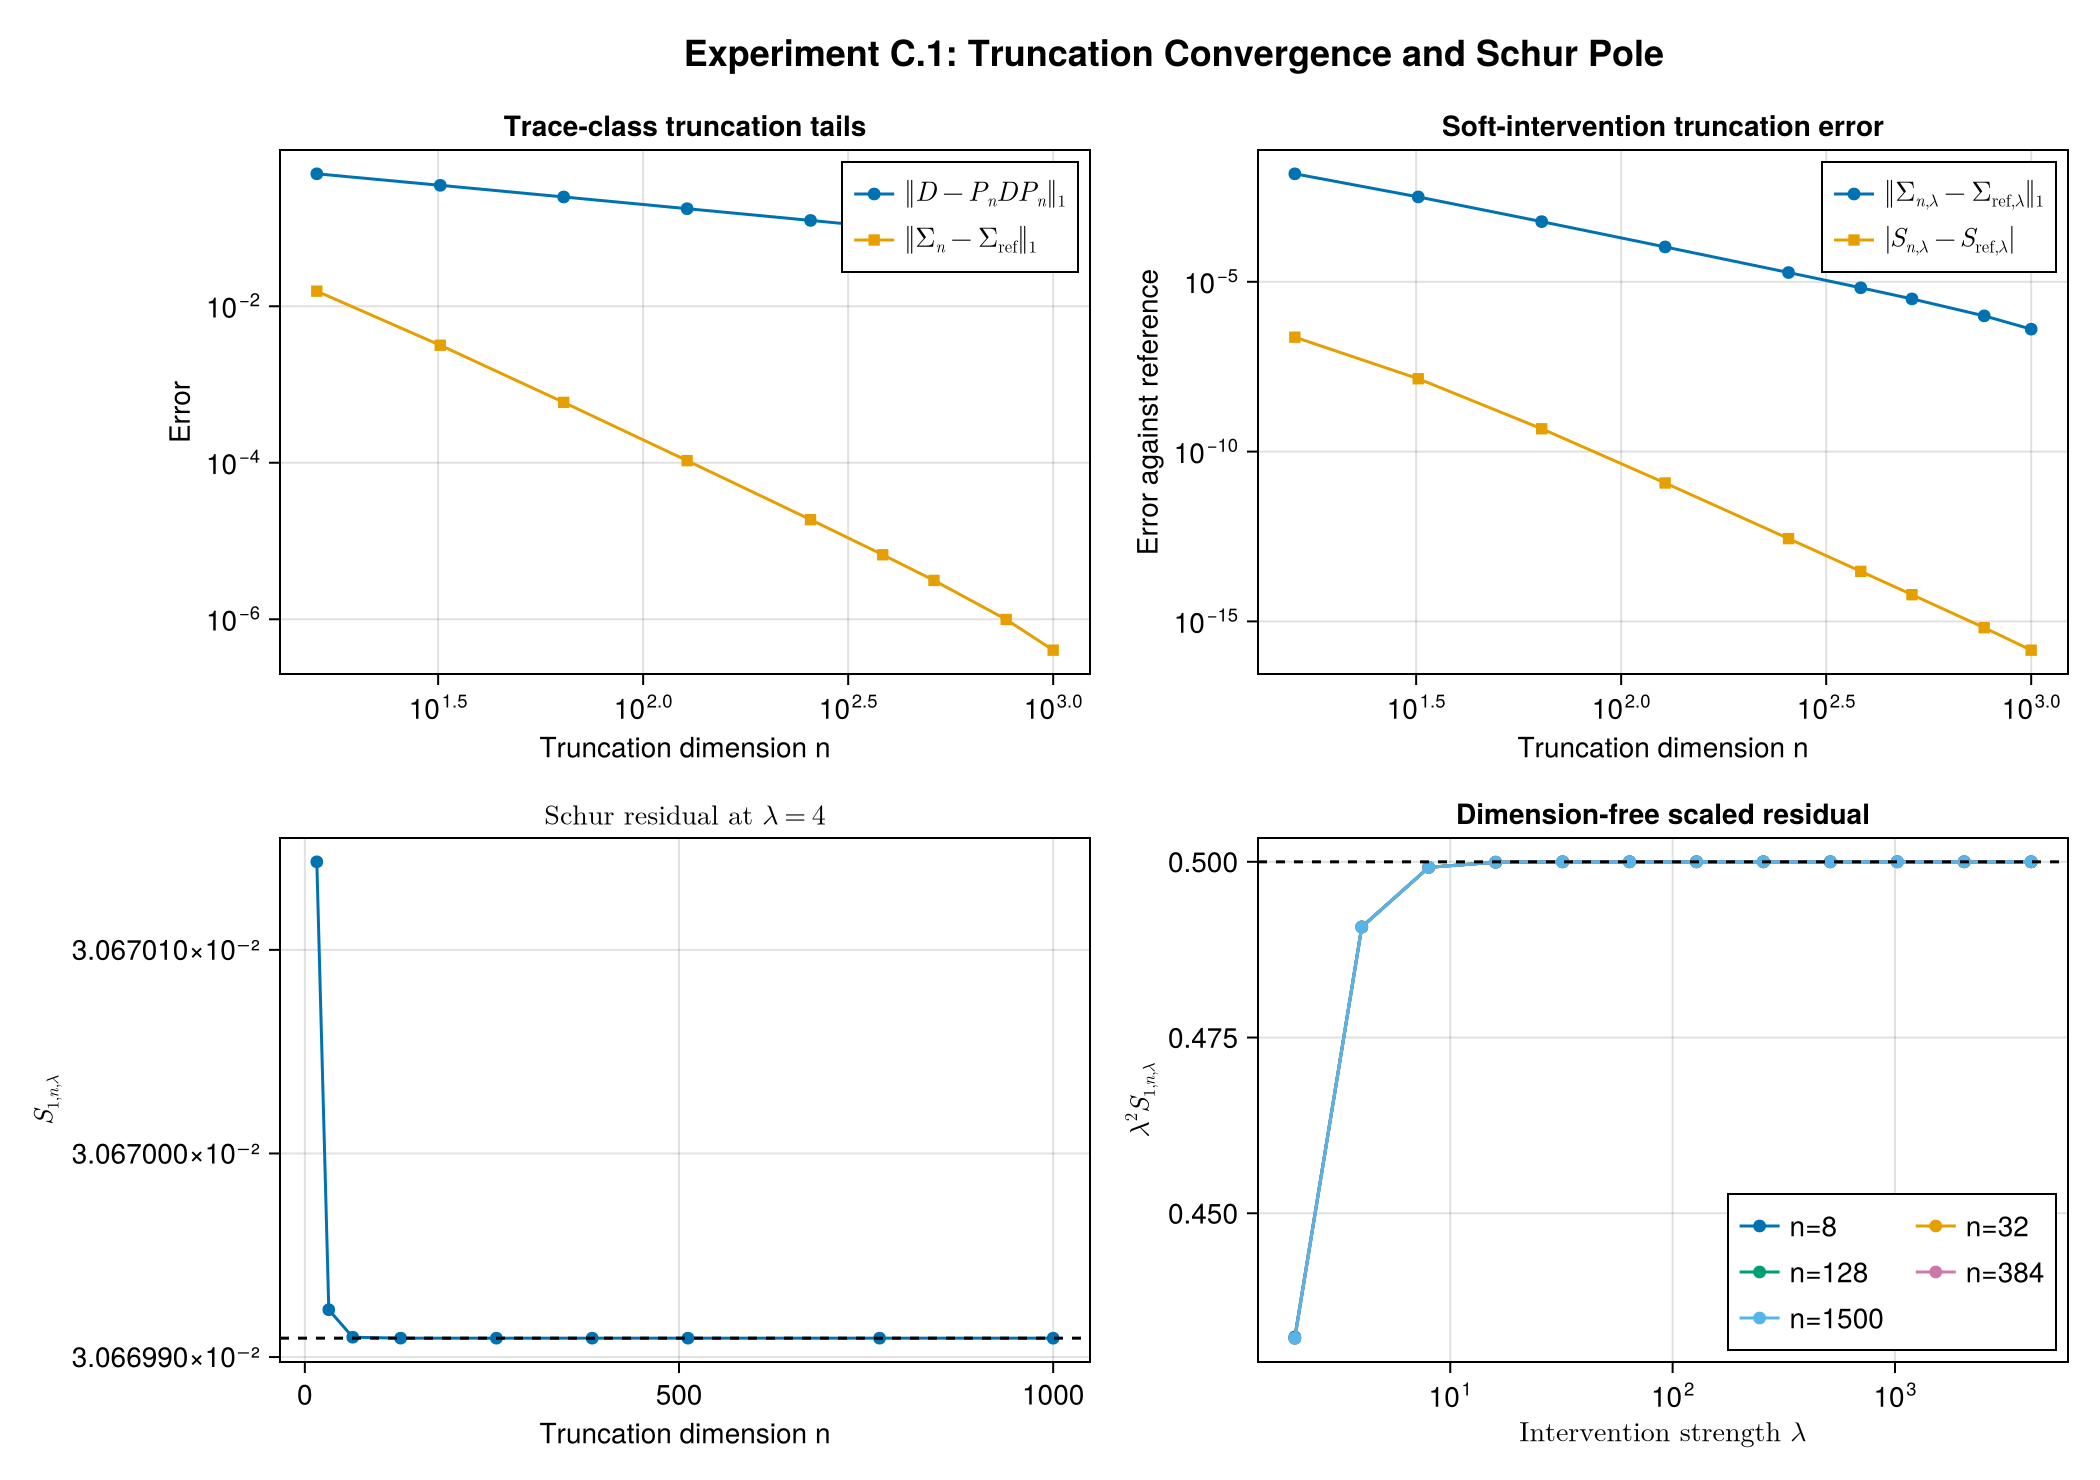
\includegraphics[width=0.8\textwidth]{figures/truncation_convergence_validation.png}
  \caption{Experiment~C.1. Trace-norm and residual errors decay in $n$; the extrapolated $m_2^{\mathrm{Schur},(1000)}$ differs from $\varepsilon_0/2$ by $6.87\times10^{-14}$.}
  \label{fig:truncation}
\end{figure}



\subsection{Exact Variance Normalization Diagnostic}
\label{app:experiments:ablation}

We validate the exact variance normalization of Proposition~\ref{prop:exact_calibration} in its decoupled reference channel. With incoming arrows cut and off-diagonal drift coupling set to zero, the target covariance is exactly $\Sigma_{\lambda,22} = d_\lambda / (2\lambda)$. Four candidate target-diffusion families are tested:
\begin{enumerate}
  \item \textbf{Canonical:} $d_\lambda=\varepsilon_0/\lambda$.
  \item \textbf{Slow:} $d_\lambda=\varepsilon_0$.
  \item \textbf{Fast:} $d_\lambda=\varepsilon_0/\lambda^2$.
  \item \textbf{Perturbed:} $d_\lambda=(\varepsilon_0/\lambda)(1+\lambda^{-2})$.
\end{enumerate}

All evaluations are performed in Julia using 256-bit \texttt{BigFloat} arithmetic. A probe at $\lambda=2^{100}$ resolves the nonzero finite-scale defect of the perturbed family.

\begin{table}[h]
  \centering
  \caption{Exact-calibration ablation. Only the canonical family satisfies the exact finite-$\lambda$ covariance condition.}
  \label{tab:ablation}
  \begin{tabular}{lll}
    \toprule
    Family & $\lambda d_\lambda/\varepsilon_0$ & defect $|2\lambda^2\Sigma_{\lambda,kk}/\varepsilon_0-1|$ \\
    \midrule
    Canonical & $1$ & $0$ \\
    Slow & $\lambda$ & $\lambda-1 \to \infty$ \\
    Fast & $\lambda^{-1}$ & $|1-\lambda^{-1}| \to 1$ \\
    Perturbed & $1+\lambda^{-2}$ & $\lambda^{-2}$ \\
    \bottomrule
  \end{tabular}
\end{table}

\begin{figure}[h]
  \centering
  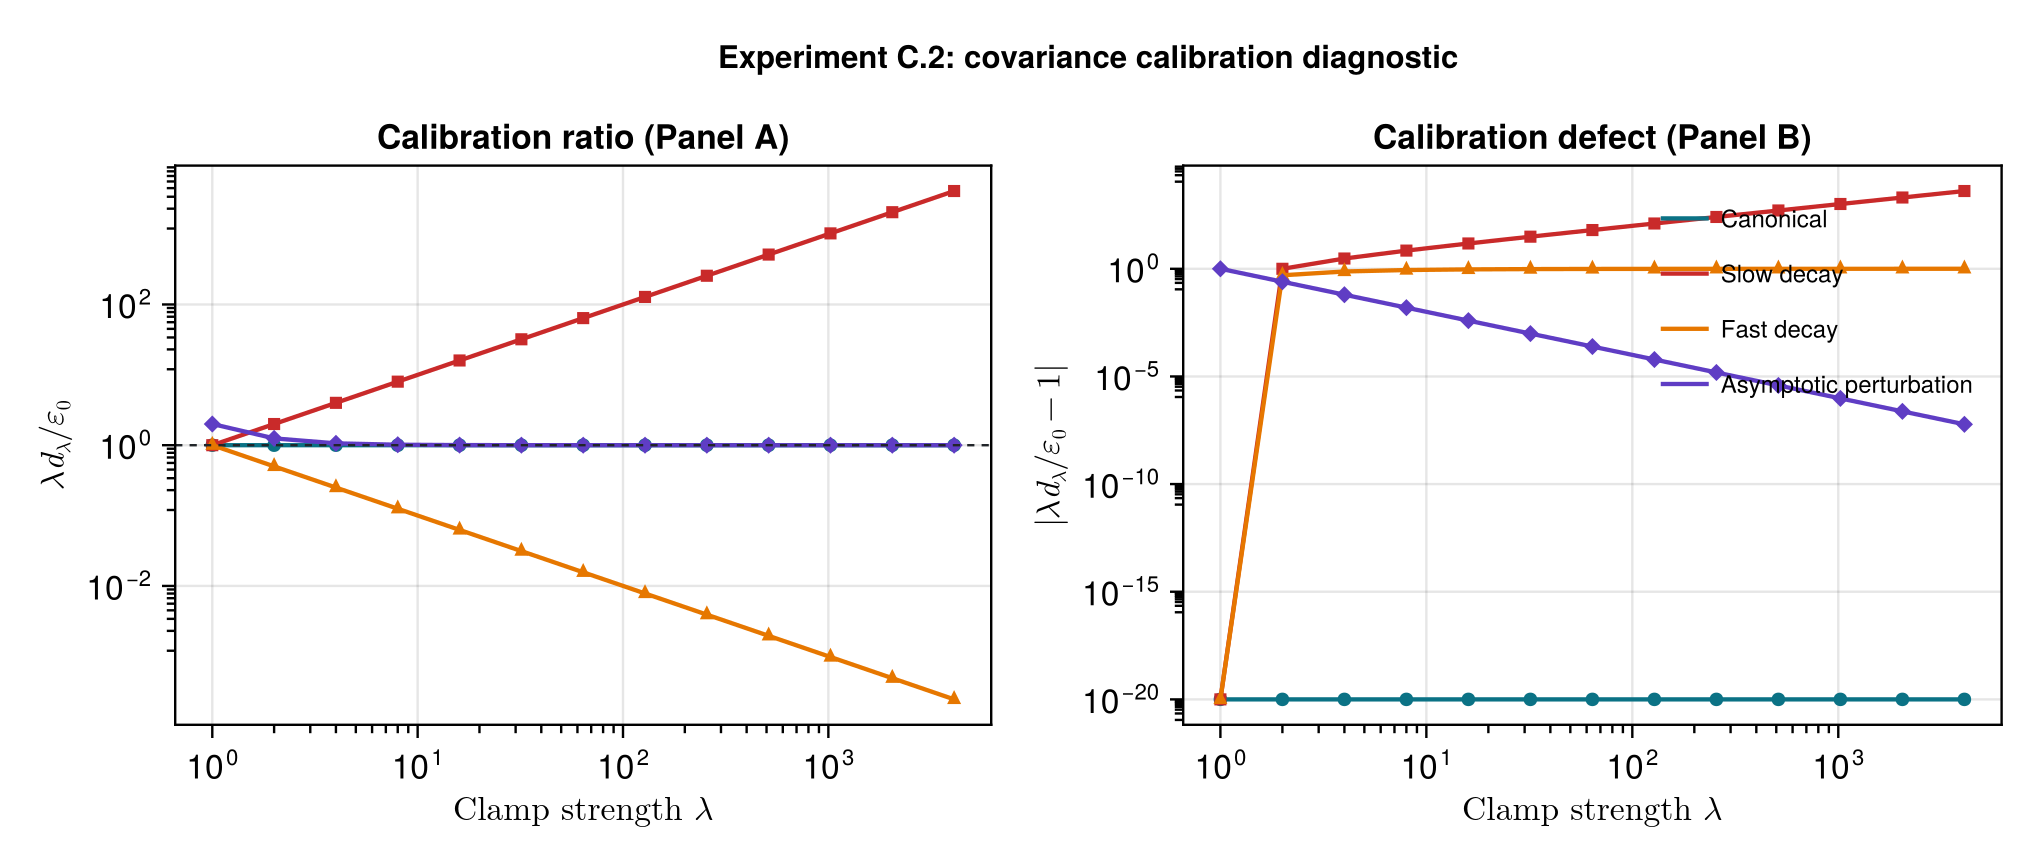
\includegraphics[width=0.9\textwidth]{figures/ablation_combined.png}
  \caption{Experiment~C.2. The perturbed family has the correct limiting ratio but fails the exact finite-$\lambda$ covariance condition. Exact zero defects are displayed at $10^{-20}$.}
  \label{fig:ablation}
\end{figure}



\subsection{Gaussian Finite-Part Functional in a Three-Node Chain}
\label{app:experiments:three_node}

We evaluate the Gaussian renormalized finite-part functional $\mathfrak{J}_\lambda$ on a three-node linear Ornstein--Uhlenbeck SDE:
\begin{equation}
  X_1 \to X_2 \to X_3,
\end{equation}
where $X_2$ is the target coordinate subject to regularized conditioning of strength $\lambda \in \{2^1, \dots, 2^{12}\}$, with $x_2^* = 0$ and $\varepsilon_0 = 1$. The drift and diffusion operators are:
\begin{equation}
  A_\lambda = \begin{pmatrix} -1 & 0 & 0 \\ 0 & -\lambda & 0 \\ 0 & a_{32} & -1 \end{pmatrix}, \qquad D_\lambda = \operatorname{diag}(1, \varepsilon_0/\lambda, 1).
\end{equation}
The target mean forcing $b_2$ controls the target mean shift $m_{\lambda,2} = b_2/\lambda$.
We evaluate three Gaussian cases:
\begin{enumerate}
  \item \textbf{Case A (Decoupled-centered):} $a_{32} = 0, b_2 = 0$. Here $\mathfrak{J}_\lambda = 0$ exactly for all $\lambda$.
  \item \textbf{Case B (Coupled-centered):} $a_{32} = 1, b_2 = 0$. The coupling causes leakage $\Sigma_{23} \neq 0$, but the centering gives $\mathfrak{J}_\lambda = O(\lambda^{-4}) \to 0$.
  \item \textbf{Case C (Coupled-off-centered):} $a_{32} = 1, b_2 = 1$. The deterministic forcing causes mean shift $m_{\lambda,2} = 1/\lambda$, yielding $\mathfrak{J}_\lambda \to b_2^2/\varepsilon_0 = 1$.
\end{enumerate}
All evaluations are performed in Julia using 256-bit \texttt{BigFloat} arithmetic, showing that the Schur residual $\lambda^2 S_{2,\lambda}$ converges to $1/2$ in all cases, while $\mathfrak{J}_\lambda$ exhibits the exact zero, $O(\lambda^{-4})$ decay, and convergence to 1 behavior respectively.

\begin{figure}[h]
  \centering
  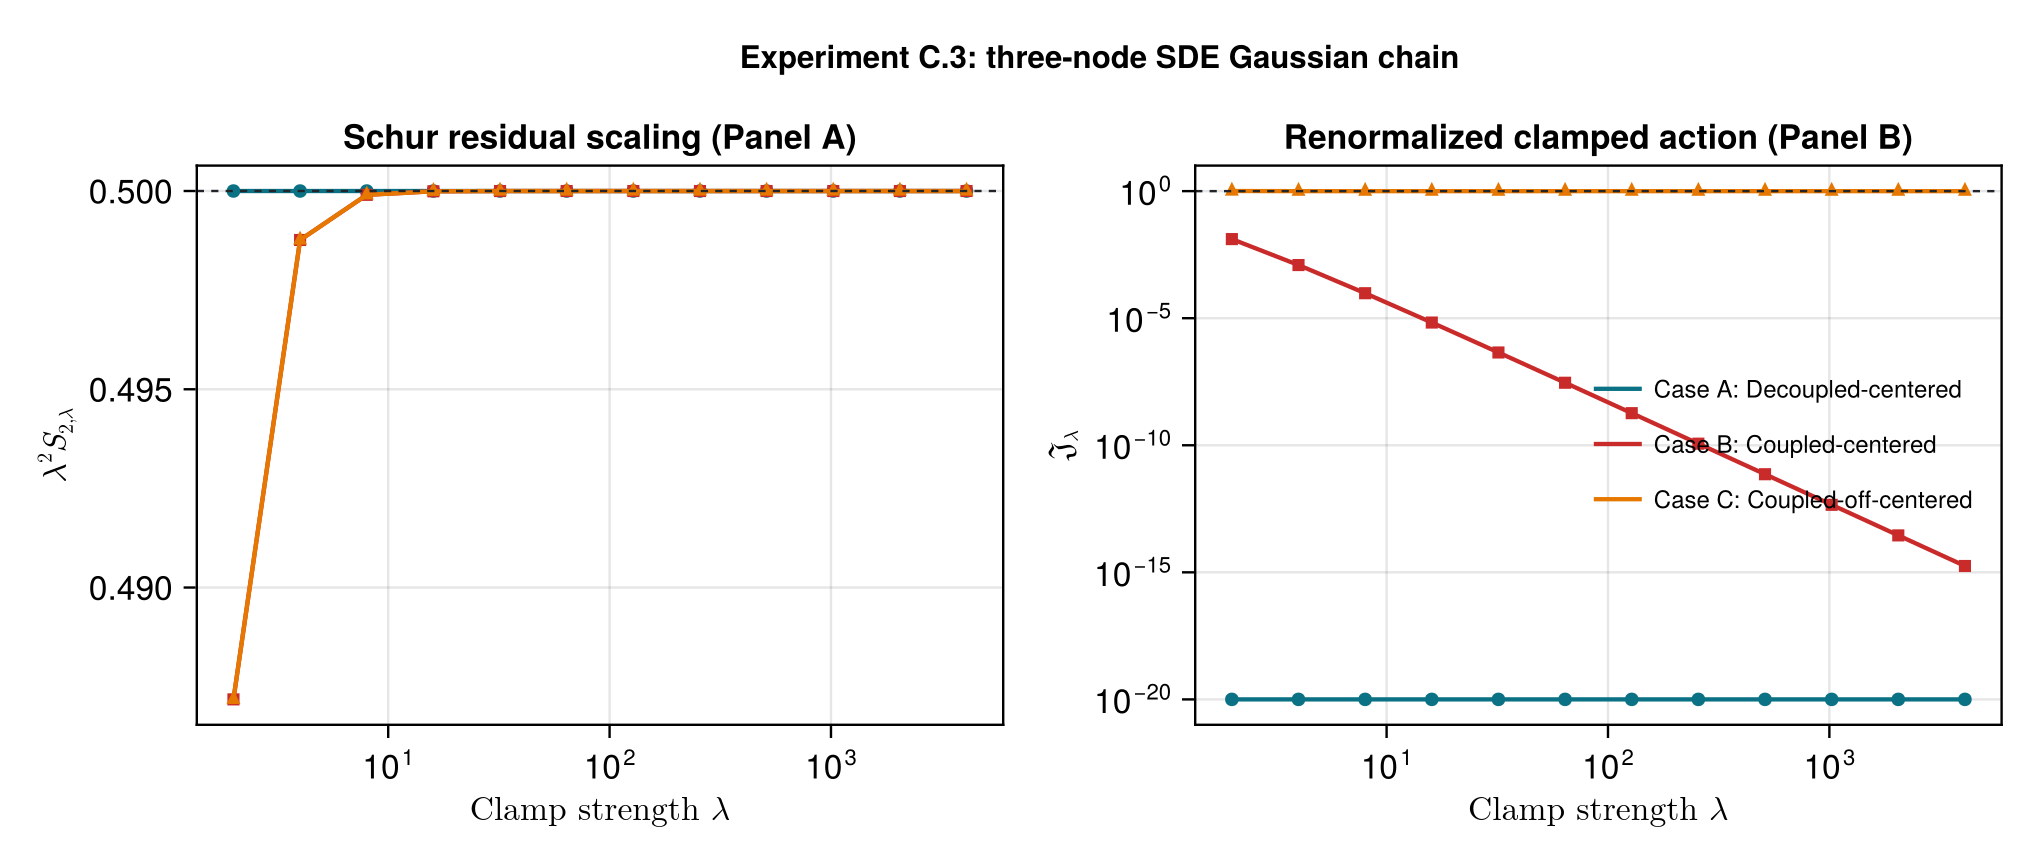
\includegraphics[width=0.9\textwidth]{figures/three_node_gaussian_chain.png}
  \caption{Experiment~C.3. The panels show $\lambda^2S_{2,\lambda}\to0.5$ and the three finite-part regimes: exact zero, $O(\lambda^{-4})$ decay, and convergence to $1$. Exact zeros are displayed at $10^{-20}$.}
  \label{fig:three_node}
\end{figure}



\subsection{Numerical Precision Audit}
\label{app:numerical_precision}

At $n=256$, we recompute representative C.1 Schur residuals using IEEE 754 \texttt{Float64} and 256-bit Julia \texttt{BigFloat} arithmetic with the same covariance equation and Schur solve.

\begin{table}[h]
  \centering
  \caption{Precision audit at $n=256$; $S_{256}$ uses 256-bit \texttt{BigFloat}.}
  \label{tab:precision_audit}
  \begin{tabular}{rrrr}
    \toprule
    $\lambda$ & $\kappa_2(\Sigma_{II})$ &
    $|\lambda^2 S-\tfrac12|$ &
    $|S_{64}-S_{256}|/|S_{256}|$ \\
    \midrule
    $4$ & $2.97\times10^6$ & $3.45\times10^{-1}$ & $6.50\times10^{-16}$ \\
    $64$ & $9.14\times10^5$ & $1.13\times10^{-3}$ & $3.48\times10^{-17}$ \\
    $4096$ & $9.14\times10^5$ & $9.20\times10^{-10}$ & $5.54\times10^{-17}$ \\
    \bottomrule
  \end{tabular}
\end{table}

For the five-point extrapolation of $m_2^{\mathrm{Schur},(256)}$,
\texttt{Float64} and \texttt{BigFloat} differ by
$9.98\times10^{-17}$; finite-$\lambda$ remainder, not rounding, governs
the observed distance to the limiting constant.



\begin{remark}[Block-decoupling error suppression]
\label{rmk:block_decoupling_error}
The sub-machine-epsilon agreement between \texttt{Float64} and \texttt{BigFloat} in Table~\ref{tab:precision_audit} is not coincidental; it is a direct consequence of the block-triangular structure established in this paper. Under the block-decoupled conditioning, the drift matrix takes the form
\begin{equation}
  \mathcal{A}^{(\lambda)}=\begin{pmatrix}-\lambda&0\\a_{Ik}&A_{II}\end{pmatrix},
\end{equation}
so the operator Lyapunov equation decomposes into three sub-problems:
\begin{enumerate}
  \item The target block $\Sigma_{\lambda,kk}=d_\lambda/(2\lambda)$ is solved by a single scalar division, incurring at most $\frac{1}{2}\epsilon_{\mathrm{machine}}$ relative rounding error (IEEE~754 round-to-nearest).
  \item The cross-covariance $\Sigma_{\lambda,Ik}$ satisfies $|\Sigma_{\lambda,Ik}|_{Q_0}=O(\lambda^{-3})$ by \eqref{eq:cross_energy_bound}, so the absolute rounding error in the cross block is $O(\lambda^{-3}\epsilon_{\mathrm{machine}})$.
  \item The free block $\Sigma_{\lambda,II}$ is a standard Lyapunov solution with absolute error $O(\epsilon_{\mathrm{machine}}\|\Sigma_{\lambda,II}\|)$.
\end{enumerate}
When the Schur complement is assembled as $S_{k,\lambda}=\Sigma_{\lambda,kk}-R_\lambda$, the subtracted variational term satisfies $R_\lambda=O(\lambda^{-6})$ (Theorem~\ref{thm:inf_cancellation}), which is negligible compared to $\Sigma_{\lambda,kk}=O(\lambda^{-2})$. The rounding error in $S_{k,\lambda}$ is therefore dominated by the error in $\Sigma_{\lambda,kk}$ alone, yielding a Schur-level rounding budget of $O(\epsilon_{\mathrm{machine}}\cdot\Sigma_{\lambda,kk})$ rather than the na\"ive $O(\epsilon_{\mathrm{machine}}\cdot\|\Sigma_{\lambda,II}^{-1}\|\cdot\|\Sigma_{\lambda,Ik}\|^2)$ that one would expect without block decoupling.

In short, the block-triangular structure converts what would be a catastrophically ill-conditioned Schur computation into a well-conditioned scalar computation plus negligible corrections. The observed \texttt{Float64}--\texttt{BigFloat} agreement at $O(10^{-17})$ is the numerical signature of this structural decoupling.
\end{remark}

\subsection{The dichotomy of dual geometries}
\label{sec:numerical:dichotomy}

To illustrate the simultaneous collapse and survival of the unified geometry under singular conditioning, we track the target scaling metrics on a 3-node serial OU chain under target coordinate conditioning on $X_2$ ($\varepsilon_0 = 1$). 
The 0th-order normal metric is extracted via the pull-back Jacobian:
\begin{equation}
  g_{\lambda,\text{normal}} := \lambda^{-2}S_{K,\lambda}^{-1}.
\end{equation}
In a log-log evaluation over $\lambda \in [2^1, 2^{20}]$, the normal metric $g_{\lambda,\text{normal}}$ instantly stabilizes to the horizontal plateau $2/\varepsilon_0$. Conversely, the unrenormalized horizontal lift response $g_\lambda^{\text{bulk}} = A_\lambda^{-2}R_\lambda$ collapses strictly at a slope of $-2$ ($O(\lambda^{-2}) \to 0$). Upon RFIM rescaling ($\lambda^2$), the 1st-order metric locks onto a distinct constant offset perfectly matching the theoretical Cameron--Martin limit $\|a_{Ik}\|_{Q_0^{-1}}^2$.

\begin{figure}[htbp]
  \centering
  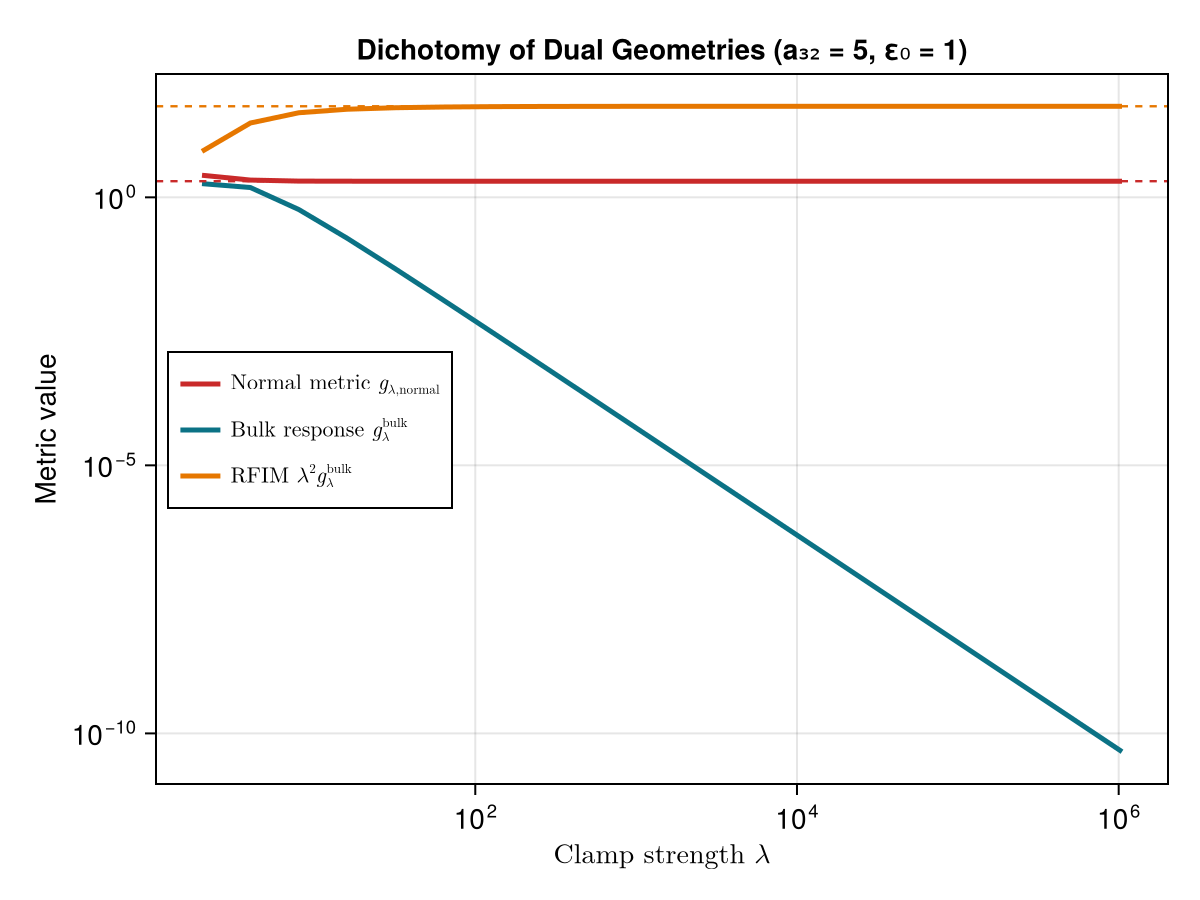
\includegraphics[width=0.75\textwidth]{figures/dichotomy_geometries.png}
  \caption{Dichotomy of dual geometries for the 3-node serial Gaussian chain under target coordinate conditioning on $X_2$ ($\varepsilon_0 = 1$, $a_{32} = 5$). The 0th-order normal metric $g_{\lambda,\text{normal}}$ (red) instantly stabilizes at the horizontal plateau $2/\varepsilon_0 = 2$, showing the survival of the boundary geometry. The unrenormalized horizontal lift response $g_\lambda^{\text{bulk}}$ (blue) collapses strictly at a slope of $-2$ as $O(\lambda^{-2})$. Rescaling the bulk response by $\lambda^2$ yields the 1st-order metric (orange), which locks onto the non-zero Cameron--Martin limit $\|a_{Ik}\|_{Q_0^{-1}}^2 = 2 a_{32}^2 = 50$.}
  \label{fig:dichotomy_geometries}
\end{figure}

The log-log scaling plot in Figure~\ref{fig:dichotomy_geometries} demonstrates that while the horizontal connection collapses, the boundary normal geometry survives intact, and the renormalized 1st-order perturbation retains the coupling invariant.



\subsection{Orthogonal independence of normal geometry and horizontal lift}
\label{sec:numerical:orthogonal}

To verify that the 0th-order boundary normal metric and the 1st-order horizontal lift quantify logically independent responses, we preserve the exact target scaling ($\varepsilon_0 = 1$) while toggling the outgoing cross-coupling $a_{32}$. 
As demonstrated in Table~\ref{tab:orthogonal_independence}, modifying the off-diagonal leakage strictly varies the 1st-order residual while leaving the normal geometry universally preserved.

\begin{table}[htbp]
  \centering
  \caption{Verification of orthogonal decoupling of normal geometry and horizontal lift}
  \label{tab:orthogonal_independence}
  \begin{tabular}{lccc}
    \toprule
    Environment & Coupling $a_{32}$ & 0th-order Metric & 1st-order Metric (RFIM) \\
    \midrule
    \textbf{Decoupled} & $0$ & $2.00000000$ & $0.00000000$ \\
    \textbf{Coupled}   & $5$ & $2.00000000$ & $49.99990463$ \\
    \bottomrule
  \end{tabular}
\end{table}

Table~\ref{tab:orthogonal_independence} numerically proves the conceptual core: the 0th-order normal metric is uniquely calibrated by the unperturbed evidence noise scale, while the 1st-order horizontal lift is exclusively governed by the off-diagonal Cameron--Martin connection energy.



\subsection{Convergence to the Mahalanobis normal well}
\label{sec:numerical:mahalanobis}

Because the background regularized-conditioning measure constitutes a Gaussian location family with covariance invariant to the evidence offset $b$, the blow-up Fisher metric matrix $G_{\lambda,K} := \lambda^{-2}S_{K,\lambda}^{-1}$ remains rigidly constant with respect to $b$ at every finite $\lambda$, yielding a purely flat geometry ($\Gamma = R \equiv 0$).
We verify the constant convergence rate of the matrix geometry in a target block of $|K|=2$. As $\lambda \to \infty$, the finite-$\lambda$ flat quadratic cost contours converge unconditionally to the limiting Mahalanobis well governed by the Schur second-order coefficient matrix $E_0$:
\begin{equation}
  \mathfrak{D}_\lambda^{\text{FP}}(b,0) = \frac{1}{2}b^\top G_{\lambda,K} b \longrightarrow \mathfrak{D}^{\text{FP}}(b,0) = b^\top E_0^{-1} b.
\end{equation}
Evaluation confirms that the distance between the intermediate geometries decays in Frobenius norm as $\|G_{\lambda,K} - 2E_0^{-1}\|_F = O(\lambda^{-4})$.

\begin{figure}[htbp]
  \centering
  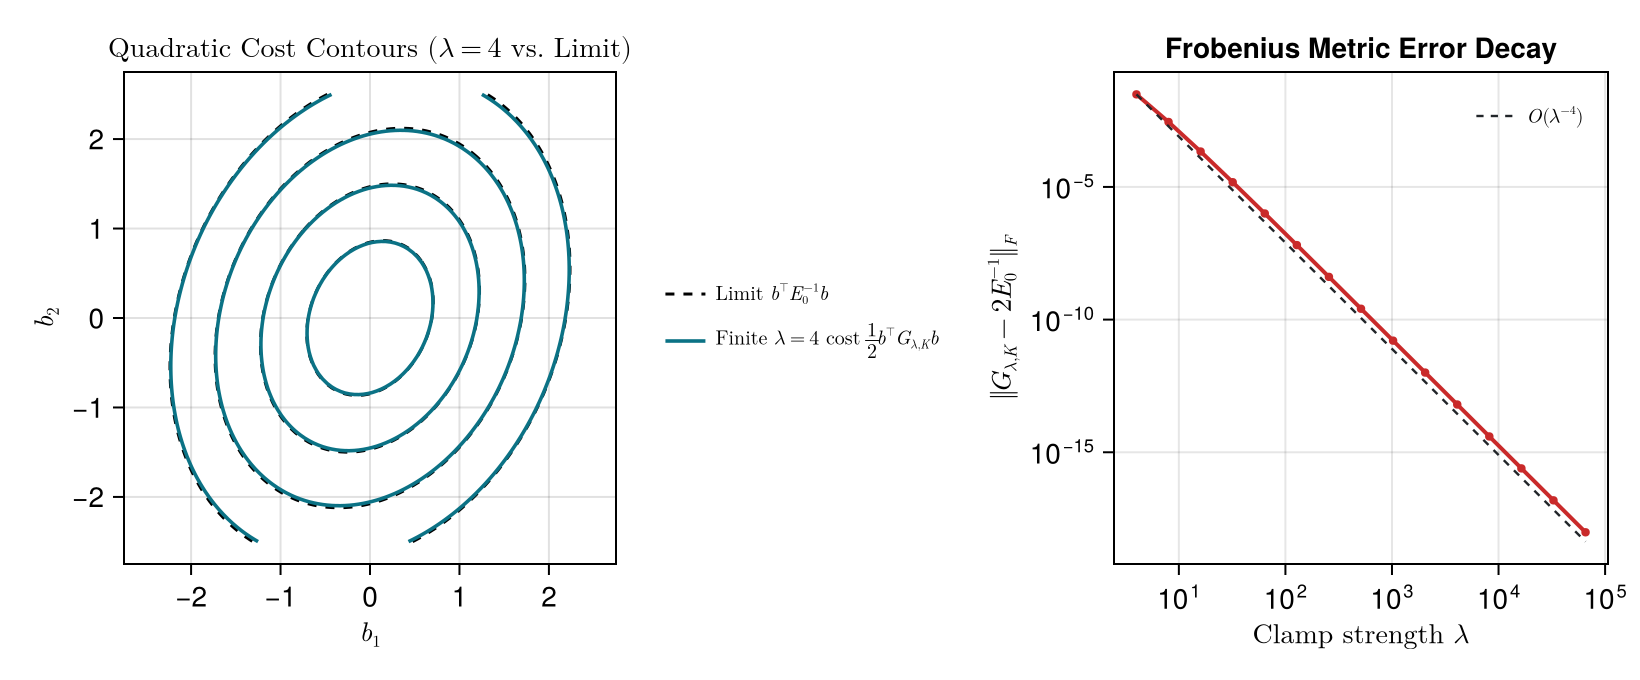
\includegraphics[width=0.95\textwidth]{figures/mahalanobis_well_convergence.png}
  \caption{Convergence of the finite-$\lambda$ quadratic cost contours to the limiting Mahalanobis normal well for target block $|K|=2$ with off-diagonal coupling. \textbf{Left (Panel A):} Contours of the finite-$\lambda$ cost $\frac{1}{2}b^\top G_{\lambda,K} b$ at $\lambda = 4$ (solid blue lines) overlaid with the contours of the limiting Mahalanobis cost $b^\top E_0^{-1} b$ (dashed black lines), demonstrating close alignment even at a low regularizer strength. \textbf{Right (Panel B):} Log-log plot of the Frobenius norm error $\|G_{\lambda,K} - 2E_0^{-1}\|_F$ (solid red line with markers) versus the regularizer strength $\lambda \in [2^2, 2^{16}]$, running in parallel with the theoretical $O(\lambda^{-4})$ slope reference (dashed black line).}
  \label{fig:mahalanobis_well_convergence}
\end{figure}

The contour comparison in Figure~\ref{fig:mahalanobis_well_convergence} (Panel A) demonstrates that the quadratic geometry of the blow-up divergence rapidly converges to the limiting Mahalanobis well. The error decay in Figure~\ref{fig:mahalanobis_well_convergence} (Panel B) confirms that the distance between the intermediate and limiting geometries in Frobenius norm decays strictly at the Schur geometric rate of $O(\lambda^{-4})$. Thus, the singularity does not generate curvature; it selects a finite flat metric. This flatness is not a vacuous triviality, but a structural consequence of the location family under regularized conditioning, with the hard-limit topological clamp rigorously preserving the displacement flatness.


